\documentclass[crop,class=article]{standalone}
%----------------------------Preamble-------------------------------%
\usepackage{tikz}           % Drawing/graphing tools.
\usetikzlibrary{
    angles,                 % Drawing angles within triangles.
    arrows.meta,            % Latex and Stealth arrows.
    quotes                  % Adding labels to angles.
}
%--------------------------Main Document----------------------------%
\begin{document}
    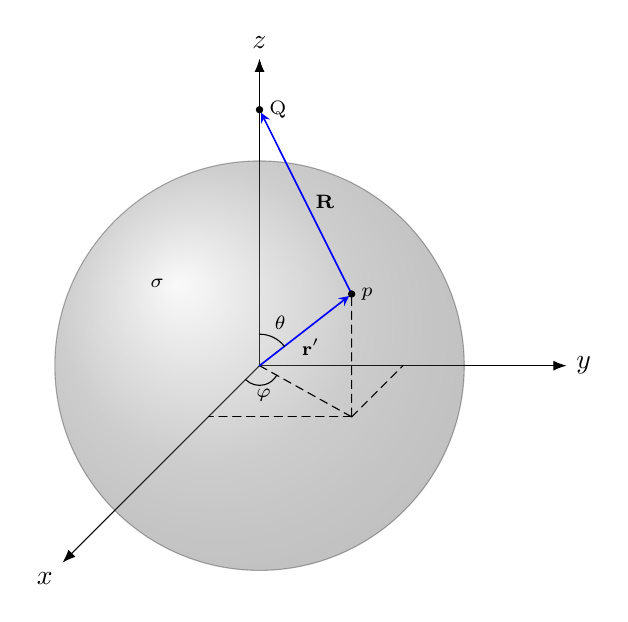
\begin{tikzpicture}[%
        line width=0.4pt,
        line cap=round,
        >={Latex},
        scale=1.3
    ]
        \draw[->] (0.0,0.0,0.0) -- (3.0,0.0,0.0) node[right] {$y$};
        \draw[->] (0.0,0.0,0.0) -- (0.0,3.0,0.0) node[above] {$z$};
        \draw[->] (0.0,0.0,0.0) -- (0.0,0.0,5.0)
            node[below left] {$x$};
        \draw[ball color=gray,opacity=0.3] (0,0,0) circle (2.0);
        \coordinate (z) at (0.0,1.0,0.0);
        \coordinate (x) at (0.0,0.0,1.0);
        \coordinate (o) at (0.0,0.0,0.0);
        \coordinate (p1) at (0.9,-0.5,0.0);
        \coordinate (p2) at (1.4,0.0,0.0);
        \coordinate (p3) at (-0.5,-0.5,0.0);
        \begin{scope}[%
            every node/.style={
                circle,
                fill=white,
                draw=black,
                inner sep=0pt,
                minimum size=2pt
            }
        ]
            \node (Q) at (0.0,2.5,0.0) {};
            \node (p) at (0.9,0.7,0.0) {};
        \end{scope}
        \node at (Q) [right] {\scriptsize{Q}};
        \node at (p) [right] {\scriptsize{$p$}};
        \node at (-1,0.8,0) {\scriptsize{$\sigma$}};
        \node at (0.5,0.18,0) {\scriptsize{$\mathbf{r}'$}};
        \draw[densely dashed] (o) -- (p1);
        \draw[densely dashed] (p) -- (p1);
        \draw[densely dashed] (p1) -- (p2);
        \draw[densely dashed] (p1) -- (p3);
        \draw[->,>=stealth,draw=blue,semithick] (o) -- (p);
        \draw[->,>=stealth,draw=blue,semithick] (p) -- node[right]
            {\scriptsize{$\mathbf{R}$}}(Q);
        \draw[fill=black] (Q) circle (0.3mm);
        \draw[fill=black] (p) circle (0.3mm);
        \pic[%
            draw=black,
            "\scriptsize{$\theta$}",
            angle eccentricity=1.5,
            angle radius= 0.4cm
        ]   {angle = p--o--z};
        \pic[%
            draw=black,
            "\scriptsize{$\varphi$}",
            angle eccentricity=1.5,
            angle radius=0.25cm
        ]   {angle = x--o--p1};
    \end{tikzpicture}
\end{document}